\documentclass[addpoints]{exam}
\usepackage{amsmath, amsfonts}
\usepackage{geometry}
\usepackage{hyperref}
\usepackage{titling}
\usepackage{tikz}
\usetikzlibrary{automata, positioning}

% Header and footer.
\pagestyle{headandfoot}
\runningheadrule
\runningfootrule
\runningheader{CS 212, Fall 2022}{HW 1: Regular Languages}{\theauthor}
\runningfooter{}{Page \thepage\ of \numpages}{}
\firstpageheader{}{}{}

\boxedpoints
\printanswers

\title{Homework 1: Regular Languages--Automata and Expressions}
\author{ungraded} % <=== replace with your team name
\date{CS 212 Nature of Computation\\Habib University\\Fall 2022}

\begin{document}
\maketitle

\begin{questions}

\question For each of the languages specified below, provide the formal specification and the state diagram of a finite automaton that recognizes it. 
  \begin{parts}
  \part[5] $L= \{w\in \{0,1\}^* \mid n_0(w)=2, n_1(w)\leq 5 \}$   where $n_x(w)$ denotes the counts of $x$s in $w$.
  \part[5] $(((00)^*(11))\cup 01)^*$.
  \end{parts}

  Please see \href{https://www3.nd.edu/~kogge/courses/cse30151-fa17/Public/other/tikz_tutorial.pdf}{this guide} for help on drawing state diagrams. \\
  \begin{center}
      \textbf{ANSWER 1A}
  \end{center}

 $L = (Q, \Sigma, \delta, Q_0, {F})$ \\
      $L = (\{q_0,1,2,3,4,5,6,7\}, \{0,1\}, \delta, q_0, \{2,3,4,5,6,7\})$ \\

  \begin{figure}[ht] % ’ht’ tells LaTeX to place the figure ’here’ or at the top of the page
    \centering % centers the figure
    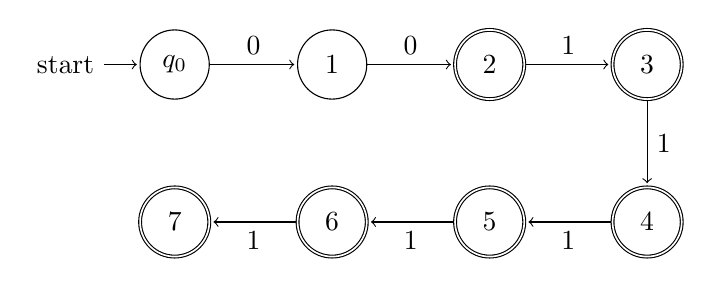
\begin{tikzpicture} [shorten >=1pt,node distance=2cm,on grid,auto] 
    
   \node[state,initial] (q_0)   {$q_0$}; 
   \node[state] (1) [right=of q_0] {$1$}; 
   \node[state, accepting] (2) [right=of 1] {$2$}; 
   \node[state, accepting] (3) [right=of 2] {$3$}; 
   \node[state, accepting] (4) [below=of 3] {$4$}; 
   \node[state, accepting] (5) [left=of 4] {$5$}; 
   \node[state, accepting] (6) [left=of 5] {$6$};
   \node[state, accepting] (7) [left=of 6] {$7$}; 
    \path[->] 
    (q_0) edge  node {0} (1)
    (1) edge  node {0} (2)
    (2) edge  node {1} (3)
    (3) edge  node {1} (4)
    (4) edge  node {1} (5)
    (5) edge  node {1} (6)
    (6) edge  node {1} (7);
    
\end{tikzpicture}
          
    \caption{Caption of the FSM}
    \label{fig:my_label}
\end{figure}

\begin{center}
    $\delta$
    \[
  \begin{array}{r|cc}
    & 0 & 1 \\\hline
    \implies q_0 &  1 & \emptyset \\
     1 & 2 & \emptyset \\
    *2 & \emptyset & 3  \\
    *3 & \emptyset & 4 \\
    *4 & \emptyset & 5  \\
    *5 & \emptyset & 6 \\
    *6 & \emptyset & 7  \\
    *7 & \emptyset & \emptyset \\
  \end{array}
  \]
\end{center}
\begin{center}
    \textbf{ANSWER 1B}
\end{center}
$L = (\{0,1, \ldots 13\}, \{0,1\}, \delta, 0, \{0,9,13\})$
\begin{center}
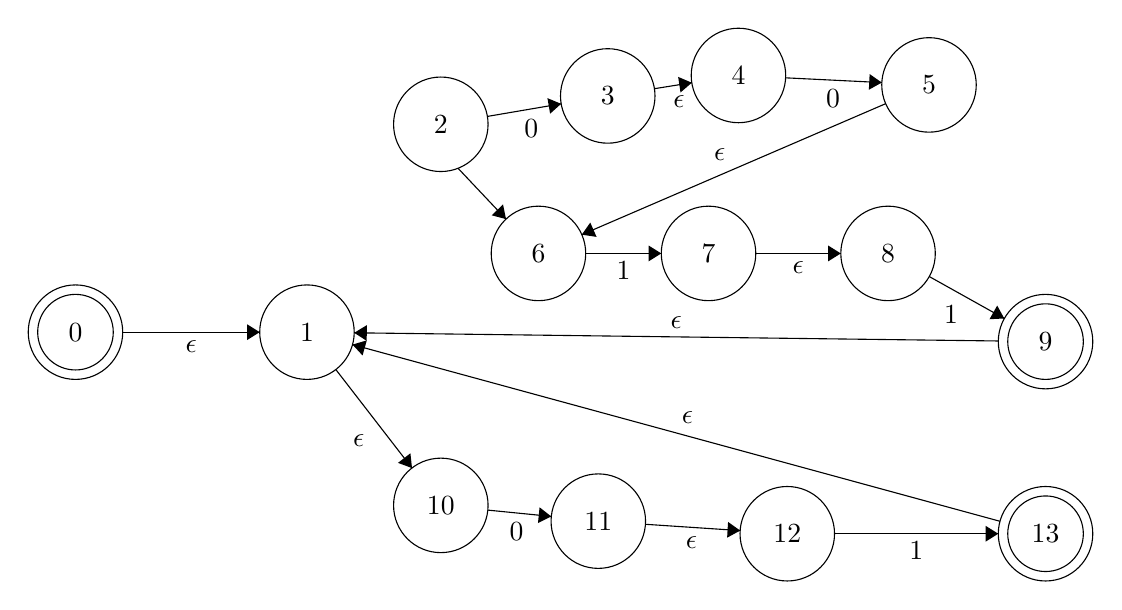
\begin{tikzpicture}[scale=0.2]
\tikzstyle{every node}+=[inner sep=0pt]
\draw [black] (9.7,-19.5) circle (3);
\draw (9.7,-19.5) node {$0$};
\draw [black] (9.7,-19.5) circle (2.4);
\draw [black] (24.4,-19.5) circle (3);
\draw (24.4,-19.5) node {$1$};
\draw [black] (32.9,-6.3) circle (3);
\draw (32.9,-6.3) node {$2$};
\draw [black] (43.5,-4.5) circle (3);
\draw (43.5,-4.5) node {$3$};
\draw [black] (63.9,-3.8) circle (3);
\draw (63.9,-3.8) node {$5$};
\draw [black] (39.1,-14.5) circle (3);
\draw (39.1,-14.5) node {$6$};
\draw [black] (49.9,-14.5) circle (3);
\draw (49.9,-14.5) node {$7$};
\draw [black] (61.3,-14.5) circle (3);
\draw (61.3,-14.5) node {$8$};
\draw [black] (71.3,-20.1) circle (3);
\draw (71.3,-20.1) node {$9$};
\draw [black] (71.3,-20.1) circle (2.4);
\draw [black] (32.9,-30.5) circle (3);
\draw (32.9,-30.5) node {$10$};
\draw [black] (42.9,-31.5) circle (3);
\draw (42.9,-31.5) node {$11$};
\draw [black] (54.9,-32.3) circle (3);
\draw (54.9,-32.3) node {$12$};
\draw [black] (71.3,-32.3) circle (3);
\draw (71.3,-32.3) node {$13$};
\draw [black] (71.3,-32.3) circle (2.4);
\draw [black] (51.8,-3.2) circle (3);
\draw (51.8,-3.2) node {$4$};
\draw [black] (12.7,-19.5) -- (21.4,-19.5);
\fill [black] (21.4,-19.5) -- (20.6,-19) -- (20.6,-20);
\draw (17.05,-20) node [below] {$\epsilon$};
\draw [black] (34,-9.1) -- (37.04,-12.32);
\fill [black] (37.04,-12.32) -- (36.85,-11.39) -- (36.13,-12.08);
\draw [black] (42.1,-14.5) -- (46.9,-14.5);
\fill [black] (46.9,-14.5) -- (46.1,-14) -- (46.1,-15);
\draw (44.5,-15) node [below] {$1$};
\draw [black] (45.89,-31.7) -- (51.91,-32.1);
\fill [black] (51.91,-32.1) -- (51.14,-31.55) -- (51.08,-32.55);
\draw (48.82,-32.46) node [below] {$\epsilon$};
\draw [black] (35.89,-30.8) -- (39.91,-31.2);
\fill [black] (39.91,-31.2) -- (39.17,-30.62) -- (39.07,-31.62);
\draw (37.71,-31.58) node [below] {$0$};
\draw [black] (26.23,-21.87) -- (31.07,-28.13);
\fill [black] (31.07,-28.13) -- (30.97,-27.19) -- (30.18,-27.8);
\draw (28.08,-26.41) node [left] {$\epsilon$};
\draw [black] (57.9,-32.3) -- (68.3,-32.3);
\fill [black] (68.3,-32.3) -- (67.5,-31.8) -- (67.5,-32.8);
\draw (63.1,-32.8) node [below] {$1$};
\draw [black] (68.41,-31.51) -- (27.29,-20.29);
\fill [black] (27.29,-20.29) -- (27.93,-20.98) -- (28.2,-20.02);
\draw (48.57,-25.34) node [above] {$\epsilon$};
\draw [black] (63.92,-15.97) -- (68.68,-18.63);
\fill [black] (68.68,-18.63) -- (68.23,-17.81) -- (67.74,-18.68);
\draw (65.3,-17.8) node [below] {$1$};
\draw [black] (52.9,-14.5) -- (58.3,-14.5);
\fill [black] (58.3,-14.5) -- (57.5,-14) -- (57.5,-15);
\draw (55.6,-15) node [below] {$\epsilon$};
\draw [black] (35.86,-5.8) -- (40.54,-5);
\fill [black] (40.54,-5) -- (39.67,-4.64) -- (39.84,-5.63);
\draw (38.65,-5.99) node [below] {$0$};
\draw [black] (46.46,-4.04) -- (48.84,-3.66);
\fill [black] (48.84,-3.66) -- (47.97,-3.29) -- (48.12,-4.28);
\draw (48.02,-4.44) node [below] {$\epsilon$};
\draw [black] (54.8,-3.35) -- (60.9,-3.65);
\fill [black] (60.9,-3.65) -- (60.13,-3.11) -- (60.08,-4.11);
\draw (57.8,-4.05) node [below] {$0$};
\draw [black] (61.15,-4.99) -- (41.85,-13.31);
\fill [black] (41.85,-13.31) -- (42.79,-13.45) -- (42.39,-12.54);
\draw (50.61,-8.64) node [above] {$\epsilon$};
\draw [black] (68.3,-20.06) -- (27.4,-19.54);
\fill [black] (27.4,-19.54) -- (28.19,-20.05) -- (28.21,-19.05);
\draw (47.85,-19.29) node [above] {$\epsilon$};
\end{tikzpicture}
\end{center}

\begin{center}
    $\delta$
    \[
  \begin{array}{r|ccc}
    & 0 & 1 & \epsilon\\\hline
    \implies *0 &  \emptyset & \emptyset & \{1\} \\
     1 & \emptyset & \emptyset & \{2,10\}\\
    2 & 3 & \emptyset & \{6\}  \\
    3 & \emptyset & \emptyset & \{4\} \\
    4 & \{5\} & \emptyset & \emptyset  \\
    5 & \emptyset & \emptyset & \{2,6\} \\
    6 & \emptyset & \{7\} & \emptyset  \\
    7 & \emptyset & \emptyset & \{8\} \\
    8 & \emptyset & \{9\} & \emptyset  \\
    *9 & \emptyset & \emptyset & \{1\} \\
    10 & \{11\} & \emptyset & \emptyset  \\
    11 & \emptyset & \emptyset & \{11\} \\
    12 & \emptyset & \{13\} & \emptyset  \\
    *13 & \emptyset & \{1\} & \{8\} \\
    
  \end{array}
  \]
\end{center}

  
\question[5] Below is the transition table of a finite automaton. $\implies$ indicates the starting state, and $*$ indicates accepting states. Provide a regular expression for the language recognized by this automaton.
  \[
  \begin{array}{r|cc}
    & 0 & 1 \\\hline
    p & \{ q \} & \emptyset \\
    \implies q & \{ q \} & \{ q, r \} \\
    *r & \emptyset & \{ s \} \\
    *s & \emptyset & \emptyset \\
  \end{array}
  \]

  \begin{center}
      \textbf{ANSWER 2 B}
      A string that will be accepted is $(0,1)^*((11)\cup (1))$ for a NFA as follows:
  \end{center}

  \begin{center}
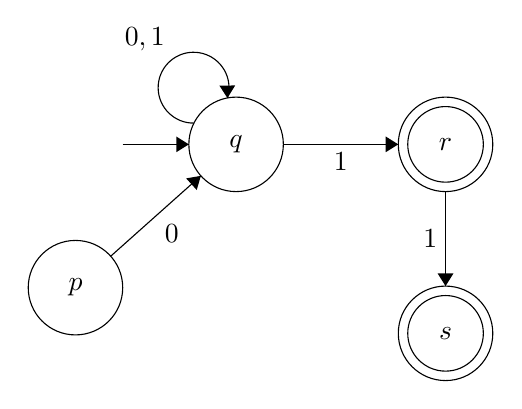
\begin{tikzpicture}[scale=0.2]
\tikzstyle{every node}+=[inner sep=0pt]
\draw [black] (19,-16.2) circle (3);
\draw (19,-16.2) node {$q$};
\draw [black] (32.3,-16.2) circle (3);
\draw (32.3,-16.2) node {$r$};
\draw [black] (32.3,-16.2) circle (2.4);
\draw [black] (32.3,-28.2) circle (3);
\draw (32.3,-28.2) node {$s$};
\draw [black] (32.3,-28.2) circle (2.4);
\draw [black] (8.8,-25.3) circle (3);
\draw (8.8,-25.3) node {$p$};
\draw [black] (22,-16.2) -- (29.3,-16.2);
\fill [black] (29.3,-16.2) -- (28.5,-15.7) -- (28.5,-16.7);
\draw (25.65,-16.7) node [below] {$1$};
\draw [black] (11.8,-16.2) -- (16,-16.2);
\fill [black] (16,-16.2) -- (15.2,-15.7) -- (15.2,-16.7);
\draw [black] (16.334,-14.85) arc (270.8699:-17.1301:2.25);
\draw (13.2,-10.3) node [above] {$0,1$};
\fill [black] (18.45,-13.26) -- (18.94,-12.46) -- (17.94,-12.47);
\draw [black] (32.3,-19.2) -- (32.3,-25.2);
\fill [black] (32.3,-25.2) -- (32.8,-24.4) -- (31.8,-24.4);
\draw (31.8,-22.2) node [left] {$1$};
\draw [black] (11.04,-23.3) -- (16.76,-18.2);
\fill [black] (16.76,-18.2) -- (15.83,-18.36) -- (16.5,-19.1);
\draw (14.91,-21.24) node [below] {$0$};
\end{tikzpicture}
\end{center}

  
  
\question
  \begin{parts}
  \part[5] Suggest regular languages $L_1$ and $L_2$ over $\{0,1\}$ such that
  \begin{enumerate}
  \item $L_1\not\subseteq L_2$,
  \item $L_2\not\subseteq L_1$, and
  \item $(L_1\cup L_2)^* = L_1^* \cup L_2^*$
  \end{enumerate}
  \part[5] Prove or disprove whether condition 3 above holds for any regular languages, $L_1$ and $L_2$.
  \end{parts}

  \begin{center}
      \textbf{ANSWER 3A}
  \end{center}
  
  Let $L_{1}$ be = ${w_{1} \in {01}^*}$ and $L_{2}$ be ${w_{2} \subseteq {10}^*}$. According to point 1 and 2, it means not all elements of either of them are present in the other one. This means not all elements of $L_{1}$ can be found in $L_{2}$ and vice versa. \\
  
  With this example, the string $w_{1}$ that will be part of language $L_{1}$ will be of the form 01s repeated and the strings $w_{2}$ that will be part of the language $L_{2}$ will be of the form 10s repeated. Hence there exist at least one such $w_{1} \not\in w_{2}$ and one such $w_{1} \not\in  w_{2}$. This shows that point 1 and 2 are true for the suggested languages.
  \\ \\
  When substitute in 3, it leads to $({01}^* \cup {10}^*)^*$. This would result in all $w_{3}$ which would be some combination of $w_{1}$ and $w_{2}$. Hence it meets the criteria for $L_{1}^* \cup L_{2}^*$.

  \begin{center}
      \textbf{ANSWER 3B}
  \end{center}

  

  

\question[5] In class, we talked about the closure of the class, $A$, of regular languages under the union, concatenation, and star operations. In this question, we want to explore whether $A$ is also closed under intersection. That is, does the following hold?
  \[
    L_1\in A \land L_2\in A \implies L_1 \cap L_2\in A
  \]

  We want to go about it as follows. The expression, $L_1 \cap L_2$, can be transformed using DeMorgan's law to an equivalent one involving union, for which closure is known, and another operation. Show whether $A$ is closed under this operation, and use your result to argue about the closure of $A$ under intersection.
   \begin{center}
      \textbf{ANSWER 4 }
  \end{center} 
  Closure under complement \\ 
  Theorem 1:\\
  The set at regular language is closed under complement. \\
  Transforming the equation we have $L_{1} \cap L_{2}$ \\ \\
     Theorem 2: \\
     The class of regular languages is closed under union operation; \\
     $L_{1} \cup L_{2}$ \\ \\
     $L_{1}' \in A$\\
     $L_{2}' \in A$ \\
    Now applying Demorgan's law: \\
    $L_{1}' \cup L_{2}' = (L_{1}' \cap L_{1}')' = L_{1} \cap L_{1} $
  \\

\question[5] We now want to explore the closure of the class, $A$, of regular languages under the operation, $mix$, which is defined as follows.
  \begin{itemize}
  \item Given strings, $u$ and $v$, both of length $n$, $mix(u,v) = u_1v_1u_2v_2\ldots u_nv_n$.
  \item Given languages, $L_1$ and $L_2$, $mix(L_1,L_2) = \{mix(u,v) \mid u\in L_1, v\in L_2, |u| = |v|\}$.
  \end{itemize}
  Is $A$ closed under $mix$? Justify your answer.
\\ \\ 
\begin{center}
      \textbf{ANSWER 5 }
\end{center} 

The approach here is to create the DFA for mix($L_1$, $L_2$) to prove that this is a regular language. To do this, we need the DFAs of $L_{1}$ and $L_{2}$. The DFA of mix($L_1$, $L_2$) (from now on referred to as $D_{mix}$) now simply has to switch between these 2 DFAs, keeping track of their states and which DFA to use to evaluate the upcoming character. This is repeated until the string terminates, and if at this point both the DFAs of $L_{1}$ and $L_{2}$ are in accept states, the string is valid.

\[D_{L_1} = (Q_{L_1}, \Sigma_{L_1}, \delta_{L_1}, q_{L_1}, F_{L_1})\]
\[D_{L_2} = (Q_{L_2}, \Sigma_{L_2}, \delta_{L_2}, q_{L_2}, F_{L_2})\]
\[D_{L_{mix}} = (Q_{L_{mix}}, \Sigma_{L_{mix}}, \delta_{L_{mix}}, q_{L_{mix}}, F_{L_{mix}})\]
\\ 

Now, we define the parameters of $D_{L_{mix}}$,

\[Q_{L_{mix}} = Q_{L_1} \times Q_{L_2} \times \{L_1, L_2\}\]
This checks out because our new $D_{L_{mix}}$ has to track all the states of $D_{L_1}$ and $D_{L_2}$, as well track of which DFA should the next input be sent to.

$\delta_{L_{mix}}$ can be defined as such,

\[\delta_{L_{mix}}((p, q, L_1), u) = (\delta_{L_{1}}(p, u), v, L_{2}),\] which basically means that if currently, $D_{L_1}$ is p, $D_{L_2}$ is q, and the next character is to be evaluated in $D_{L_1}$, then $L_1$ state is changed to $\delta_{L_{1}}(p, u)$ when u is read, and state of $L_2$ remains the same. \\Similarly,
\[\delta_{L_{mix}}((p, q, L_2), v) = (p,\delta_{L_{2}}(q, v), L_{1}),\]

\[q_{L_{mix}} = (q_{L_{A}}, q_{L_{b}}, L_1)\]
which basically means that $D_{L_{mix}}$ starts with $D_{L_{1}}$ in $q_1$, $D_{L_{2}}$ in $q_2$, and then switches back to $D_{L_{1}}$.

\[F_{L_{mix}} = F_{L_1} F_{L_2} L_{1}\]
which essentially means that the entire string is accepted if both $D_{L_1}$ and $D_{L_2}$ are in accept states and the next character is set to be evaluated in $D_{L_1}$ (because we have set it up this way).



  
\end{questions}

\end{document}

%%% Local Variables:
%%% mode: latex
%%% TeX-master: t
%%% End:
